\addcontentsline{toc}{section}{\textbf{Summary}}
\begin{abstract}
Data analytics and verification is a subset of Avionics within the Aurora V Rocketry team, representing RMIT University in the 2024 Australian Universities Rocket Competition (AURC). Work conducted within this subsystem makes up the Capstone project with the aim to design, test, and validate data analytics for the avionics, ground communications, redundant electronic and payload systems. The aim of this proposal is to offer background research and a high-level overview of the methodologies and risks that are involved. The project will span across the launch of five Aurora Rocket, with each providing an opportunity to collect and analyse sensor data. From an analysis and verification perspective, previous Rocketry project have used techniques such as Kalman Filters and Sensor fusion for post flight data processing. Similar techniques will likely be employed for data analysis. Lastly, a number of risks and ethical considerations have been identified to ensure the responsible implementation of data analytics and verification processes.  
\end{abstract}

\section{Problem statement}
The Data Analytics and Verification team is to operate as a subset within the AURC Avionics Team for the HIVE Aurora V rocket project. This subsystem's primary objective is to design, test, and validate data analytics processes for the avionics, ground communications, redundant electronic systems, and payload systems.  

The project scope spans across five iterations of the Aurora rocket (A1 through to A5). As each rocket iteration progresses, data analysis processes should change to improve the accuracy of verification processes. Feedback during analysis is also to be provided to the broader Avionics team.     

\subsection{Project Deliverables}
Data analytics and verification processes will include:  
\begin{itemize}
  \item Data Capture and Logging Design: Defining sampling rates and intervals for data capture and establishing data logging and storing formats. 
  \item Real-Time Processing: Research and develop algorithms for sensor fusion to integrate data from multiple sensors. Implement filtering techniques to remove noise. 
  \item Post-Processing: Perform statistical analysis to evaluate key performance metrics of avionics systems. Implement systems to detect deviations from expected behaviour when comparing raw sensor and fused data to the data captured by the blue raven.     
  \item Data Visualization: Develop tools for generating informative graphs and charts for data interpretation. Explore the possibility of creating simulations based on collected data. 
  \item Data Validation: Determine the validity of the captured data. Identify the nature of errata (error with our analysis methods or hardware issue?) 
\end{itemize}


\subsection{Tools to Undertake Data Analytics and Verification}
Due to the nature of work, most tools will be software based. The processor of the microcontroller will influence which integrated development environment (IDE) will be used. Tools such Arduino IDE, Visual Studio IDE and Microchip studio will most likely be utilized for development. Although the use of code libraries should be avoided to maintain low level control of the avionics system, some libraries may be utilized to act as a starting point. For version control and collaboration, Git will be used throughout the course of the project. A list of tools that will be required to complete the project includes:

\begin{itemize}
  \item Git version control
  \item Integrated Development Environments including Arduino and STM32CubeIDE
  \item Arduino and Python libraries for prototyping, testing, and offline data processing 
  \item Embedded systems analysis tools such as debug probes and logic analysers
\end{itemize}

\section{Background and literature review}\label{sec:lit-review}
The Aurora V project aims to build a L3 rocket designed to fly with apogee at exactly 30,000ft. To achieve this goal, accurate data collection and analysis is a necessity both to understand the flight path of the rocket and its contributing factors to facilitate correcting modifications to the rocket itself, as well as to supply real-time state information to the airbrake system for dynamic adjustments to drag coefficients.

Inertial sensors are susceptible to noise in their measurements, which introduces error into captured data and accumulates a drift in time-varying calculations. Many model rockets such as Pioneer Rocketry's Skybreaker\cite{pioneer-rocketry} implement some variation of a Kalman Filter to smooth out this noise for more accurate state estimation. A Kalman Filter attempts to provide an accurate estimation for noisy processes by using a model in combination with previous estimates to predict the future state of the process, correcting this prediction with measured data\cite{kalman-introduction,kalman1960}. This process accounts for the process noise - deviation between the true state of the process and the state as described by the model - as well as the noise generated by the measurement of state values. A Kalman gain is computed to weight how much of the modeled and measured data should be accounted for in the new estimate, with an error covariance matrix tracking the uncertainty in the estimate.

Rockets built by university teams such as uORocketry and NTNU generally make use of positional data such as height or displacement together with velocity measurements to control their airbrake systems\cite{uORocketry, NTNU}. To accurately determine these state variables, sensor fusion techniques may be employed to reduce the accumulated error that results from the measurement process. 

An example of how this may be applicable is in the altitude calculations. The most simple method of determining altitude would be to directly use the barometric pressure, however this is highly dependant on calibration at the launch site and susceptible to noise introduced from the sensor. An alternative would be to use integrated accelerometer data to obtain position, however the process of integrating itself is prone to drift due to time lag as well as flight angle offsets. A potential solution for these problems would be to combine the barometric altitude estimate together with positional calculations from the integrated accelerometer data, as described in a 2004 report by David Schulz\cite{kalman-apogee}. Accelerometer data can also be combined together with gyroscopic measurements from the IMU to rotate the inertial frame, allowing for pure vertical acceleration data to be integrated down to positional information. In all cases, some application of a Kalman filter appears necessary.


\section{Research questions}
\begin{questions}
  \item What variables are necessary to track in the rocket state?
  \item What algorithms should be run to accurately estimate rocket state in real time (e.g. linear vs. extended Kalman Filter)?
  \item How will sensor fusion techniques be applied to obtain state information from available data? \begin{questions}
    \item What data from available sensors should be combined to state data?
  \end{questions}
  \item What statistical analysis techniques will be employed to assess real time validity of data? \begin{questions}
    \item What communication protocols will be used to inform the redundant systems of detected errata?
    \item What metric(s) will the redundant systems use to elect which of primary and secondary sensors to sample?
  \end{questions}
  \item What visualisation methods will be applied to provide state representation in real time?
  \item What visualisation methods will be applied to provide state information offline? \begin{questions}
    \item What techniques will be applied to analyse trends in offline data? 
    \item What trends are important to analyse in offline data?
  \end{questions}
\end{questions}

\section{Methodology}
This section of the proposal focuses on the preparations that have been made to ensure the success of the project, outlining current design work and how it will enable further developments in the future. A brief discussion on time management and resource planning is provided, followed by a functional breakdown of the higher level design goals and on-board processes for data analytics and verification within the avionics subsystem. 

Additionally, some insight into the structure and handling of data both in real-time and offline are provided towards the end of this section.

\subsection{Time planning}
Appendix~\ref{apdx:gantt} provides a proposed timeline for this project. As of submission of this proposal, testing for data sampling firmware has begun ahead of the Aurora I launch and is on track to be completed on time. Following this submission, the next steps are to begin development on the data processing firmware and analysis software for later launches.

\subsection{Resource planning}
This project team consists of two students, Jeremy Timotius and Matthew Ricci with Dr Glenn Matthews as the project supervisor. As this team operates alongside the Avionics (ground communications and redundant systems) team, members of this team will serve as an ongoing resource. 

Collaboration between the two teams will take place regularly through in person and online meetings. Other members from different subsystems may also be engaged as their skill set may be relevant to avionics. From a software perspective for data analysis, RMIT student licenses and laboratory computers will be utilized to perform project work.  

\subsection{Functional breakdown}
The high-level flow chart shown in Figure~\ref{fig:flowchart-high_level} depicts how raw sensor data is to be captured and transmitted from a firmware perspective. The purpose of the flow chart is to guide avionics on how data is to be logged and transmitted to enable post flight analysis and verification. The system is primarily broken down into a high-resolution interval at 500Hz and low-resolution interval at 50Hz. 

These resolution intervals are intended to match with Blue Raven intervals in order to sync and compare data sets post flights. The Blue Raven data will act as a benchmark to determine the accuracy of data collected from various sensors of the avionics unit. Logging of data will be triggered based on a launch event recorded from the Blue Raven to enable both systems to collect data simultaneously. 

During flight, captured sensor data will be written to an onboard flash memory and transmitted over LoRa to ground communications, providing a level of redundancy to mitigate the risk of data loss. This dual approach ensures that if one method encounters failure or interruption, data can still be processed and analyzed post flight. 

While flash memory can only be analyzed post flight, LoRa communications provides critical live communications to the ground, enabling real-time monitoring and analysis of sensors and microcontrollers. Real-time processing through the use of algorithms is to be developed with the purpose of detecting hardware failures and or abnormalities to inform avionic systems to switch to redundant sensors or microcontrollers if required.  

\begin{figure}[h]
  \begin{center}
    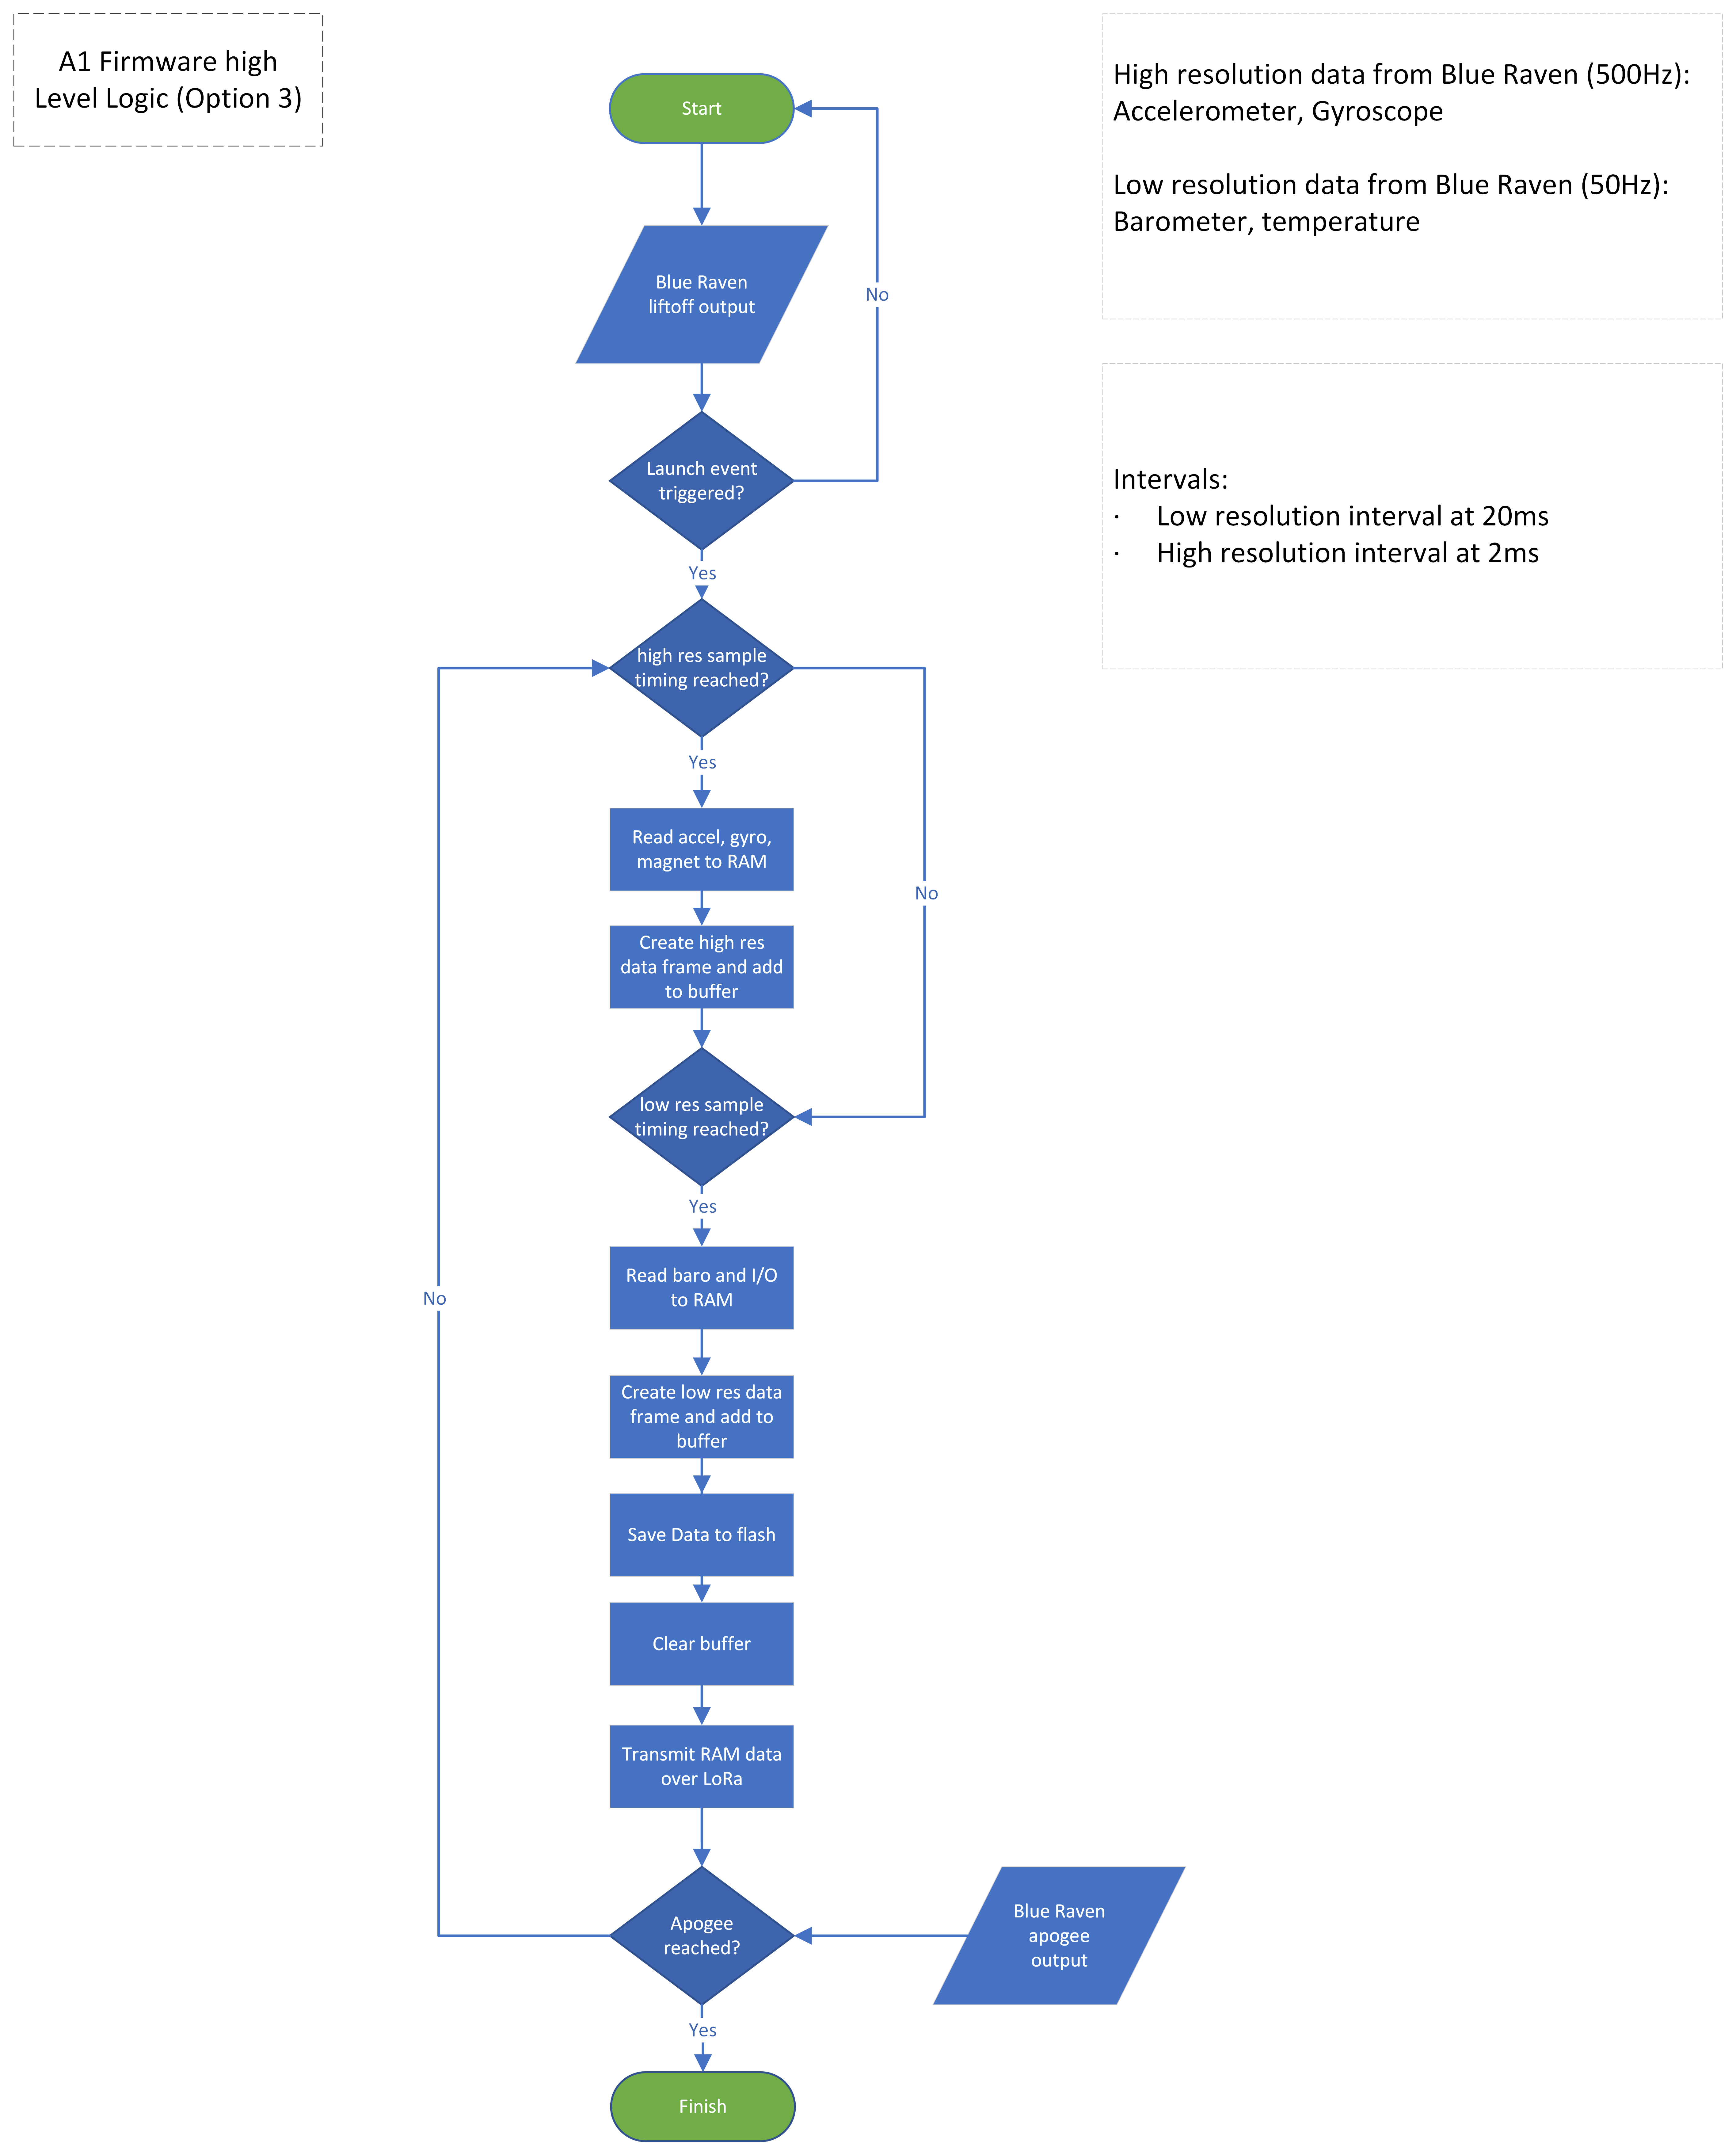
\includegraphics[width=0.95\textwidth]{img/flowchart-high_level.png}
  \end{center}
  \caption{High-level functional flowchart of data sampling and logging}\label{fig:flowchart-high_level}
\end{figure}

The design outlined in Figure~\ref{fig:flowchart-high_level} is focused solely on the capture, storage, and transmission of data. During flight, real-time processing algorithms will additionally be run to combine the raw sensor data and provide accurate and relevant data for the airbrake subsystem control.

During the high-resolution interval, the system reads data from an IMU (Inertial Measurement Unit) which consists of an accelerometer, gyroscope, and magnetometer sensors. These sensors are essential in determining the aircraft motion and orientation; therefore, a higher sampling rate is required to capture subtle changes accurately. Raw data from sensor registers are then combined with header to form a data frame which will be stored in a buffer array ready to be stored in flash. Sensor data will additionally be kept in RAM to be transmitted during the low-resolution interval.  

At the low-resolution interval, the system reads data from a barometer, which includes a pressure and temperature sensor to determine altitude. Similar to the high-resolution interval, raw data are used to form a data frame which is added to a buffer array serving as temporary storage before the data is written to flash. Once pressure and temperature data frame is formed and saved to RAM, the buffer array is written to flash and data stored in RAM will be transmitted over LoRa. Switch I/O will also be written to RAM and transmitted to ground control to notify avionic systems if a switch has turned off.  

A number of alternate design methods were considered which included a separate logging interval where transmission and saving to flash occurred over a separate time frame. Although having a different interval provides greater control, flash writing and LoRa transmission occurring during on the low-resolution interval simplifies the design, consolidating data handling tasks.  

\subsection{Data storage and handling}
To facilitate data processing post flight, data retrieved from sensors must be logged in a structured format to allow the host system to recognise the type of data being read. This involves determining the structure of dataframes being stored to flash, as well as designing a method for the host to interpret these dataframes. In addition, it is important that data is correctly synchronised both with internal datasets, as well as the data collected by the Blue Ravens. For all these problems, inspiration was taken from the Blue Raven to provide a solution that was applicable to this project.

\subsubsection{Dataframe structure}\label{sec:dataframe-structure}
Figure~\ref{fig:dataframe-structure} provides a bytefield structure for the dataframes being constructed from the on-board avionics sensors. Each frame contains a two-byte header that identifies the type of data recorded in the payload (e.g. high resolution, low resolution or rocket payload data), describes the number of bytes contained within the payload, and provides a synchronisation byte for post processing.\\[0.5em]

\begin{figure}[h]
  \begin{center}\hspace{4.5em}
  \begin{bytefield}[bitwidth=2em, endianness=big]{8}
    \bitheader{0,5,6,7}\\
    \begin{rightwordgroup}{Header}
      \bitbox{2}[bgcolor=bittersweet]{ID} 
      \bitbox{6}[bgcolor=aquamarine]{length}\\
      \wordbox{1}[bgcolor=aquamarine]{Sync} 
    \end{rightwordgroup}\\
    \begin{rightwordgroup}{Payload}
      \wordbox{1}{$D_0$[15:8]}\\
      \wordbox{1}{$D_0$[7:0]}\\
      \wordbox{1}{$D_1$[15:8]}\\
      \wordbox[lrt]{1}{}\\
      \cskippedwords{blue!20}\\
      \wordbox[lrb]{1}{}\\
      \wordbox{1}{$D_n$[7:0]}
    \end{rightwordgroup}
  \end{bytefield}
  \end{center}
  \caption{Dataframe structure for avionics}
  \label{fig:dataframe-structure}
\end{figure}

These dataframes will be stored within a \verb|uint8_t| buffer as opposed to a 16-bit equivalent. This is because some sensor data is contained within 24 bits per sample, so to make efficient use of space while maintaining simplicity of implementation 8-bit nibbles are desirable.

\subsubsection{Data typing}\label{sec:data-typing}
Data stored by the avionics system will retain the raw structure as output by the on-board sensors, written as 8-bit unsigned blocks. This is to minimise the amount of storage used with each frame, as well as to avoid any processing overhead from computing real data. 

Processing can then be done offline during analysis to obtain real data, for example by multiplying out the sensitivity of a given sensor into a floating point variable.

\begin{figure}[h]
  \begin{center}\hspace{4.5em}
  \begin{bytefield}[endianness=big]{16}
    \bitheader{0,15}\\
    \begin{rightwordgroup}{X-axis}
      \bitbox{8}[]{Upper nibble} 
      \bitbox{8}[]{Lower nibble} 
    \end{rightwordgroup}\\
    \begin{rightwordgroup}{Y-axis}
      \bitbox{8}[]{Upper nibble} 
      \bitbox{8}[]{Lower nibble} 
    \end{rightwordgroup}\\
    \begin{rightwordgroup}{Z-axis}
      \bitbox{8}[]{Upper nibble} 
      \bitbox{8}[]{Lower nibble} 
    \end{rightwordgroup}
  \end{bytefield}
  \end{center}
  \caption{Example structure for a single sensor payload}
  \label{fig:payload-structure}
\end{figure}

The payload of each dataframe will consist of consecutive groupings of sensor data, an example of which is pictured in Figure~\ref{fig:payload-structure}. No delimiter will be used to separate these groupings and instead processing will be performed by using an agreed upon structure. 

Code that processes this data will need to read in each dataframe from memory, using the length field in the header to delimit where the data ends. Based on the type information from the frame header, each variable of data can then be read.

\section{Synchronisation}\label{sec:synchronisation}
According to the Blue Raven user's guide \cite{adamson_2023}, synchronisation between high and low resolution data is achieved through a "sync code" that is stored with the data. This code is essentially a counter that increments with each millisecond, wrapping at a count of 250. 

To maintain synchronisation both with datasets collected by Aurora V avionics, as well as with the Blue Raven data (for the sake of comparison), an identical solution will be implemented within the logging system. As outlined in Section~\ref{sec:dataframe-structure}, this sync code is presented as a full byte in the frame header, following the id and frame length. This byte will be included with all forms of saved data to maintain synchronisation parity across the board.

\subsection{Mid-flight and post processing}
Data collected through the previously discussed methods will be used for processing both during the flight and on recovery. On-board filtering and fusion algorithms as mentioned in Section~\ref{sec:lit-review} will be developed to provide the airbrake system the necessary state data for controls. It is important that these algorithms are performant to minimise impact on logging and transmission during flight. Alternative solutions will also be considered, such as isolating the processing of data to prioritise data logging through scheduling systems, or vice versa if appropriate. 

Data transmitted to the ground mid-flight will also require some real time processing and visualisation to provide the team with feedback while the rocket is off the ground. This will require a visualisation framework such as NASA's OpenMCT\cite{about}, as well as ground processing of data taking advantage of the increased computing power to provide further insight than what will be available from the rocket directly.

Leading up to the launch of Aurora V, data will be collected from previous rocket launches during the project. This data will be crucial in the development of data processing and validation software, allowing for insight to be gained in the performance of developed algorithms through comparison to the Blue Ravens. This data will also be necessary in the development of these algorithms in the first place, as the data can be analysed to provide information on the rocket's state model as well as the noise performance of the measurements to be applied within the filtering system.

\section{Risk assessment}
From an occupational health and safety perspective, the risks associated with this project are minimal. Due to the nature of this project, most risks will be office related, which include, visual strain, neck, and back pain from long hours in front of computers causing eye strain, headaches, and fatigue. Although these risks pose health concerns, they can be effectively managed through ergonomic interventions such as the use of ergonomic furniture and regular breaks during project work. Additionally, some aspects of testing verification will include interaction with hardware such as sensors and other electronic modules. 

While these interactions may introduce physical hazards such as the risk of electrical shocks or injury from handling equipment, hardware is to be handled in RMIT Laboratory rooms where proper procedures and PPE will be utilized. Hardware will also be regularly inspected and maintenance to help identify and address potential safety hazards proactively.  

As data analysis and verification is heavily reliant on the avionic hardware, there are foreseeable risks that may impact how data analysis and verification is approached. Table~\ref{tbl:risk} outlines possible risks and contingency strategies to ensure project deliverables are met.  

\begin{table}[h]
\centering
\begin{tabular}{>{\raggedright}p{4cm}p{1.5cm}p{1.5cm}p{7cm}}
\toprule
\textbf{Risk} & \textbf{likelihood} & \textbf{Impact} & \textbf{Contingency Strategy} \\ \midrule
Delay arrival of avionic hardware & High & High & \vspace{-1.5em}
\begin{itemize}[leftmargin=*]
  \item Work closely with Avionics team to understand if there are any Hardware changes or substitutions.
  \item Prioritise non hardware dependent tasks.
  \item Focus on preliminary data analysis, algorithm development, or simulation testing while awaiting hardware arrival.
\end{itemize}\\\midrule
Data collected from sensors is corrupted or incomplete & Medium & High & \vspace{-1.5em}
\begin{itemize}[leftmargin=*]
  \item Develop an algorithm for data validation and error detection to identify and filter out unreliable data.
\end{itemize}\\\midrule
Loss of ground communication during flight & Medium & High & \vspace{-1.5em}
\begin{itemize}[leftmargin=*]
  \item Testing processes to ensure that data can be extracted from flash.
\end{itemize}\\\midrule
Flash data unrecoverable & Medium & High & \vspace{-1.5em}
\begin{itemize}[leftmargin=*]
  \item Ensure that enough senor data is being transmitted in both high- and low-resolution transmissions. This will still enable data analysis to take place even if flash data is lost.
\end{itemize}\\\midrule
Scope creep & Low & Medium & \vspace{-1.5em}
\begin{itemize}[leftmargin=*]
  \item Establish clear project scope.  
  \item Prioritise data analysis and verification task.  
  \item Regularly review project scope and assess proposed changes with Glenn Matthews.
\end{itemize}\\\midrule
Integration Challenges with ground communication and real-time processing & Medium & Medium & \vspace{-1.5em}
\begin{itemize}[leftmargin=*]
  \item Understand the specifications between the communication hardware and processing algorithm. 
  \item Conduct integration checks and testing.
\end{itemize}\\
\bottomrule
\end{tabular}
\caption{Risk assessment}\label{tbl:risk}
\end{table}

\subsection{Ethical considerations}

As this project is primarily focused on data analysis and verification through software, ethical considerations are minimal. However, due to the nature of the aerospace and the work conducted, some considerations are as follows.   

Although the test flights and the official AURC competition are held in controlled environments with safety precaution in place, the real-time data logged through LoRa may play a factor in identifying a potential safety risk.  

Over the course of multiple Aurora flights, a large amount of data will be collected and stored. It should be ensured that the data and analysis should be only used for its intended purposes. As this work is conducted under RMIT and the HIVE association, these stakeholders should be consulted before data is shared externally. 

The Aurora team is made of five subsystems with a total of over thirty members from different backgrounds and walks of life. Ethical collaboration is essential to ensure that all team members are treated with respect and have equal opportunities to contribute to the project. Open communication among team members should be encouraged to create a culture of inclusivity. 


